\documentclass[conference]{IEEEtran}

\usepackage{amsmath,amssymb}
\usepackage{cite}
\usepackage{graphicx}
\usepackage{textcomp}
\usepackage[table]{xcolor}
\usepackage{url}
\usepackage{array}

\newcolumntype{L}[1]{>{\raggedright\arraybackslash}p{#1}}

\begin{document}

\title{AprilCube: 3D-Printable Fiducial Targets for \\Reliable 6-DoF Pose Estimation}

\author{\IEEEauthorblockN{Younghyo Park}
\IEEEauthorblockA{MIT\\
Cambridge, MA}
}
\maketitle

\begin{abstract}
AprilCube is an open-source toolkit for generating 3D-printable fiducial targets and estimating their six degree-of-freedom pose from camera images. The repository couples a multi-material 3MF generator with a detector that uses the same configuration file to recover the three-dimensional corner position of every marker. It supports both parametric cuboids and voxel-composed targets specified as unions of axis-aligned cuboids or occupied voxel grids, enabling T-shapes, frames, chairs, stair targets, and other non-box geometries. This paper describes the software artifact, its geometry model, generated print and simulation assets, pose-estimation pipeline, streaming API, and synthetic validation harness. The project is intended as a reproducible physical tracking target for robotics, calibration, simulation, and interactive vision experiments.
\end{abstract}

\begin{IEEEkeywords}
fiducial marker, pose estimation, 3D printing, voxel target, robotics, software
\end{IEEEkeywords}

\section{Introduction}
Planar fiducial systems such as ArUco and AprilTag provide robust local features for camera pose estimation \cite{aruco,apriltag}. They are widely used because the printed target is cheap, the visual code carries an identifier, and off-the-shelf detectors can localize marker corners accurately. A single planar marker or board, however, exposes only one plane of three-dimensional structure. It can leave the camera view under rotation, become ambiguous when viewed from near-frontal single-marker configurations, and lose many correspondences when the target is partially occluded.

AprilCube addresses this by turning the marker board into a printable three-dimensional object. Markers are placed on exposed surfaces of a known target, and every marker corner is represented in a common object coordinate frame. As the object rotates, different surfaces become visible, but the detector can aggregate all visible corners into a single Perspective-n-Point (PnP) problem. The target therefore behaves less like a flat calibration sheet and more like a small tracked object that can be grasped, moved, placed in a robot workspace, or loaded into a simulator.

The repository contains two tightly coupled components. The generator produces printable targets, model previews, and simulation assets. The detector consumes the generated configuration and estimates the target pose from images or video. This shared data model is the central design choice: the printed artifact, the detector, and the simulation mesh are all derived from the same marker dictionary, physical cell size, margins, borders, tag identifiers, and target geometry. For cuboids, the geometry can be reconstructed analytically from the grid. For non-cuboids, the configuration stores explicit marker-corner coordinates.

\begin{figure}[t]
\centering
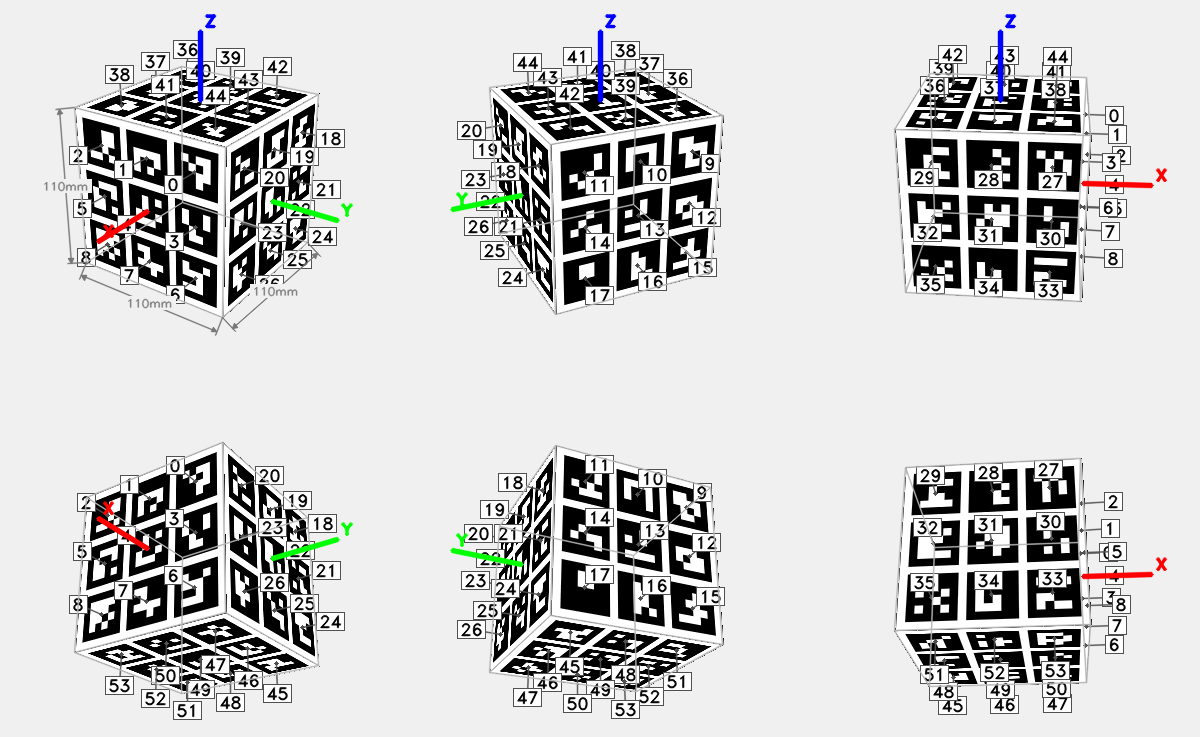
\includegraphics[width=0.94\linewidth]{aprilcube_overview_cropped.png}\\[-0.15em]
\scriptsize\textbf{(a)} Generated model preview\\[0.45em]
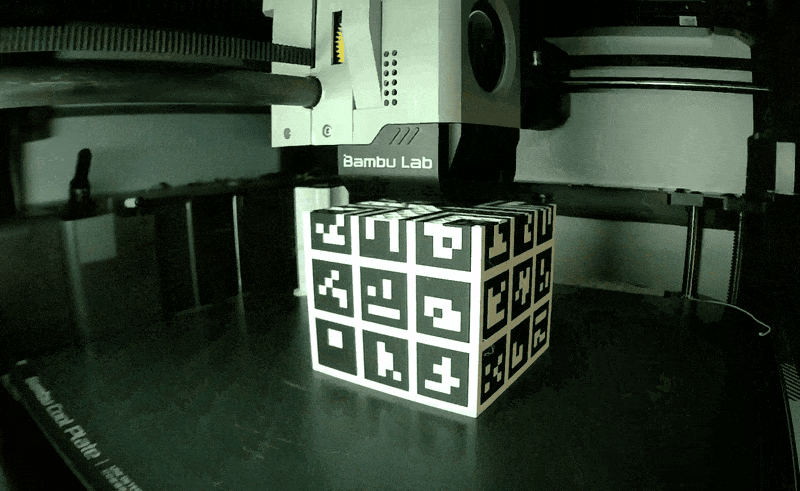
\includegraphics[width=0.94\linewidth]{printing_process_still.png}\\[-0.15em]
\scriptsize\textbf{(b)} 3D printing still
\caption{AprilCube couples a generated fiducial target model with a printable physical artifact. (a) The generator renders marker identifiers and object-frame axes. (b) A still frame from the repository GIF shows the marker pattern being fabricated on a dual-material FDM printer.}
\label{fig:overview}
\end{figure}

The generator supports two target families. Parametric cuboids provide a compact default. Voxel-composed targets are specified in YAML as the union of one or more axis-aligned voxel cuboids or as an explicit occupied voxel grid, after which one marker is placed on each exposed voxel face. Together, these target families support both cube-like tracking props and shape-rich targets whose silhouette, graspability, or visibility profile can be chosen for a particular robotics experiment.

The main contributions are:
\begin{itemize}
\item a generator for ArUco/AprilTag cuboids and voxel-composed targets with configurable grids, tag sizes, margins, borders, marker identifiers, and YAML geometry specifications;
\item an asset pipeline that emits multi-color 3MF files, detector JSON, preview images, textured OBJ assets, and MuJoCo MJCF models from the same geometry;
\item a Python detector that reconstructs exact 3D marker-corner positions from analytic cuboid layouts or explicit per-marker records, aggregates multi-face observations, solves robust PnP, filters video poses, and exposes synchronous, asynchronous, and visualization-oriented APIs;
\item a synthetic benchmark harness that renders ground-truth target poses, applies degradations such as occlusion and blur, and checks pose error across systematic viewpoints and trajectories.
\end{itemize}

\begin{figure}[t]
\centering
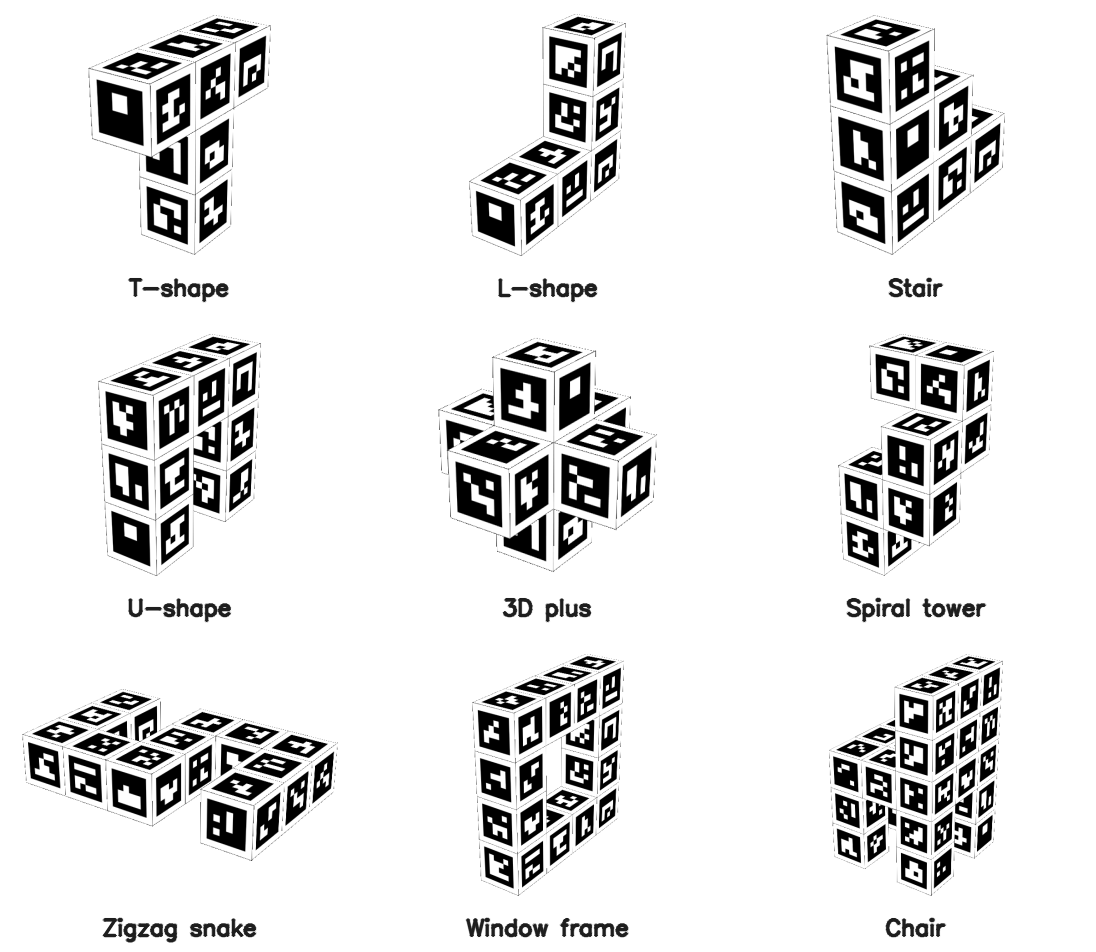
\includegraphics[width=\linewidth]{voxel_shape_gallery.png}
\caption{Voxel-composed example targets generated from YAML specifications. Each exposed voxel face carries one marker, and the detector configuration records the marker-corner coordinates explicitly.}
\label{fig:voxel_gallery}
\end{figure}

\section{Design Goals}
AprilCube was designed around the practical workflow of making a physical target, printing it, and then using it in camera-driven robotics software without manually transcribing geometry. The first goal is self-description: every printed object has a configuration file that fully specifies the dictionary, tag identifiers, dimensions, and face layouts. The second goal is consistency across media: the 3MF, preview image, OBJ mesh, MJCF model, and detector all use the same object coordinate frame. The third goal is graceful degradation in video: the detector should provide useful estimates when only a subset of faces is visible, when one or two detections are poor, or when a short burst of frames is temporarily lost.

These goals make the repository closer to a reproducible instrument than to a collection of scripts. The user can regenerate a target, print an already-generated model, load the same target into simulation, and run the detector with the same JSON file. This is especially useful for small projects where tracking hardware, motion-capture systems, or carefully manufactured calibration rigs are too expensive or cumbersome, but where a planar printed marker is too fragile a pose reference.

The design also favors inspectability. Generated thumbnails display the marker identifiers, face geometry, and object axes before fabrication. The detector reports visible faces, tag ids, inlier counts, reprojection error, and a debug overlay in addition to the pose. Those diagnostics are intentionally simple because many failures in fiducial tracking are practical failures: the camera is out of focus, the print contrast is poor, the wrong configuration file was loaded, or the marker is viewed at an angle where only a small number of corners remain reliable.

\section{Repository Artifact}
AprilCube is packaged as a Python project with a command-line entry point, a public Python API, generated model assets, examples, and synthetic tests. The core runtime dependencies are NumPy and OpenCV's contributed ArUco module \cite{opencv}. Optional visualization uses viser and the textured OBJ model exported by the generator.

The repository includes 37 generated model directories: 28 cuboids and nine voxel-composed targets. The cuboids cover one to ninety total tags, with tag sizes from 12 mm to 30 mm and side lengths from 30 mm to 180 mm. The voxel targets include T-, L-, U-, stair-, plus-, spiral-, serpentine-, frame-, and chair-like shapes. Each model directory stores a multi-color 3MF file, a detector configuration file, a rendered preview, and MuJoCo-compatible assets. This model zoo is useful in two ways: users can print a target without first learning the generator options, and the checked-in outputs serve as examples of the exact file bundle produced by the code.

The public package interface is intentionally small. Users can call \texttt{aprilcube.detector()} with either a model directory or a configuration file, plus camera intrinsics as a JSON file, dictionary, or 3-by-3 matrix. The returned estimator processes OpenCV frames and reports pose, reprojection error, visible faces, detected tags, and optional visualization overlays. The command-line interface exposes generation and webcam-oriented workflows for users who do not need to write Python code.

\begin{table}[t]
\caption{Main repository artifacts}
\label{tab:artifacts}
\centering
\begingroup
\footnotesize
\renewcommand{\arraystretch}{1.18}
\setlength{\tabcolsep}{4pt}
\arrayrulecolor{black!35}
\rowcolors{2}{black!4}{white}
\begin{tabular}{@{}L{0.34\columnwidth}L{0.57\columnwidth}@{}}
\rowcolor{black!13}
\textbf{Artifact} & \textbf{What it contributes} \\
\hline
\texttt{generate.py} & Parametric cuboid geometry, voxel-cuboid YAML parsing, marker textures, 3MF writing, thumbnail rendering, OBJ and MJCF export. \\
\texttt{detect.py} & Marker detection, 2D--3D aggregation, PnP pose solve, temporal filtering, overlays, async processing, and viser integration. \\
\texttt{models/*\_cube/} & Pre-generated printable and simulation-ready cubes and cuboids. \\
\texttt{models/*\_target/} & Voxel-composed targets with explicit per-marker geometry records. \\
\texttt{test\_detection.py} & Synthetic renderer, discrete viewpoint checks, trajectories, video output, and image degradations. \\
\texttt{examples/} & Webcam, web-based visualization, and YAML target specifications. \\
\hline
\end{tabular}
\rowcolors{2}{}{}
\arrayrulecolor{black}
\endgroup
\end{table}

\section{Parametric and Voxel Target Generation}
For cuboids, the generator takes a marker dictionary, tag identifiers, a grid size \(g_x \times g_y \times g_z\), and either tag size or cell size. The grid describes how many markers lie along the object axes rather than how many markers lie on one particular face. This makes rectangular cuboids natural: a \(5\times4\times1\) target, for example, becomes a flat box with large top and bottom faces and narrow side strips, while a \(3\times3\times3\) target becomes a conventional cube.

A marker with dictionary bit width \(d\) occupies
\begin{equation}
m = d + 2
\end{equation}
cells after including its one-cell black border. With border \(b\), inter-tag margin \(s\), and \(n\) tags along one object axis, the total number of cells along that axis is
\begin{equation}
a(n)=2b+nm+\max(0,n-1)s.
\end{equation}
The physical dimensions are then \(c[a(g_x),a(g_y),a(g_z)]\), where \(c\) is the cell size in millimeters. The total number of required markers is
\begin{equation}
N=2(g_xg_y+g_xg_z+g_yg_z).
\end{equation}

The six faces are assigned stable outward normals and face-local ``right'' and ``down'' directions. The convention is chosen so that the cross product of the face-local right and down axes equals the outward normal. This convention is used in three places: texture layout, mesh triangle winding, and detector-side corner reconstruction. Because all three are derived from the same face definitions, the rendered preview, the exported simulation mesh, and the detector agree on the object frame.

Voxel targets replace the global cuboid grid with an occupancy set \(V \subset \mathbb{Z}^3\). In the YAML interface, \(V\) can be specified as a union of axis-aligned integer cuboids or as an explicit voxel grid. A voxel face receives a marker when its neighboring voxel in the outward normal direction is empty. The number of markers is therefore
\begin{equation}
N_V=\sum_{p\in V}\sum_{f\in \{\pm x,\pm y,\pm z\}}\mathbf{1}[p+n_f \notin V],
\end{equation}
where \(n_f\) is the unit neighbor offset for face direction \(f\). The bounding dimensions are the occupied voxel extent multiplied by the voxel size. This simple rule is sufficient to create the examples in Fig.~\ref{fig:voxel_gallery}, including targets with holes, concavities, overhang-like silhouettes, and multiple disconnected-looking exterior patches that are still face-connected through the voxel body.

The YAML schema separates geometry, marker, size, layout, and material settings. A \texttt{voxel\_cuboids} target stores a list of integer cuboids with \texttt{origin} and \texttt{size}; a \texttt{voxel\_grid} target can enumerate occupied voxels directly. Both paths share dictionary selection, identifier ranges, tag or cell size, border cells, material inversion, and output location. This keeps simple cuboids scriptable from command-line flags while allowing more expressive targets to be checked into the repository as readable specifications.

The generator writes a configuration JSON that maps every marker identifier to physical geometry needed by the detector. For cuboids, this includes the dictionary name, grid, tag identifiers, per-face id layout, cell size, tag size, margins, borders, and box dimensions. For voxel targets, the JSON additionally stores one record per marker containing its voxel index, face direction, outward normal, face corners, and marker corners in millimeters. The detector does not infer the printed geometry from the image; it reconstructs it exactly from this JSON.

For physical fabrication, the project writes 3MF files with Bambu Studio paint-color attributes so white cells can be assigned to a second extruder on dual-material printers. The mesh is constructed at cell resolution: black cells are part of the base material, while white cells are marked with the alternate paint color. This keeps the output compatible with slicer workflows that expect a single 3MF package rather than separate STL shells.

For simulation and visualization, the same face textures are packed into texture atlases and exported as Wavefront OBJ, MTL, and MJCF files for MuJoCo \cite{mujoco}. Cuboids use a compact atlas over the six box faces, while voxel targets use atlases over their exposed marker faces. The exported OBJ uses meter units and an object frame consistent with detector output. The MJCF file adds a textured visual mesh and collision geometry, making the target convenient for simulated robotics scenes where the visual marker pattern and physical collision shape should be aligned.

\section{Fabrication Workflow}
The intended fabrication workflow begins with either a cuboid grid or a YAML target specification, plus a dictionary choice. Small cubes such as \(1\times1\times1\) or \(2\times2\times2\) are compact physical props, while larger grids provide more visible tags and therefore more PnP correspondences. Flat boxes such as \(5\times4\times1\) behave like thick marker boards with side markers that keep the object observable under roll or pitch. Voxel targets add another design axis: the user can choose a silhouette or physical affordance, such as a frame, chair, or stair shape, while still retaining exact marker geometry in the detector configuration. The generator checks that the requested dictionary contains enough unique identifiers and then writes the complete output directory.

The 3MF output is meant to be opened directly in a slicer that understands material assignment attributes. In a typical dual-color FDM workflow, the base material is black and the painted cells are white. The choice is conventional rather than mathematical: the detector ultimately sees image contrast. In practice, matte materials, adequate lighting, and a camera exposure that avoids clipping the white cells matter more than the exact brand of filament.

Because the marker pattern is part of the physical geometry, the generated dimensions should be treated as the design specification rather than as a guarantee of the printed object. Slicer settings, extrusion width, nozzle diameter, layer height, elephant-foot compensation, support strategy, bridging behavior, and surface finish can all perturb marker corners. This is especially relevant for expressive voxel targets, which may contain concave regions or tall thin members. The repository therefore emphasizes reproducibility of the digital artifact and leaves metrological validation to the user's printer and camera setup.

\section{Pose Estimation Pipeline}
The detector first loads the JSON configuration and reconstructs a map from marker id to its four three-dimensional corner coordinates. Cuboid configurations are reconstructed from the grid and face definitions; voxel-target configurations can provide the corner map directly through the per-marker records written by the generator. The corner order matches OpenCV's marker convention, so image corners can be paired directly with object-space corners. For every frame, the detector converts the image to grayscale, applies contrast normalization, detects ArUco or AprilTag-compatible markers with tuned OpenCV parameters, filters detections to the target's known id set, and aggregates all observed marker corners into a single 2D--3D correspondence set.

The OpenCV detector parameters are tuned for the visual properties of multi-material 3D prints. The accurate preset uses sub-pixel corner refinement, a wide adaptive-threshold window range, relaxed candidate perimeter limits, and dense perspective sampling. A faster preset reduces threshold passes and skips sub-pixel refinement for webcam use. The detector also includes a fallback pass with sharpening and relaxed decoding when the primary detector finds no valid markers, which helps recover frames affected by motion blur or poor contrast.

Given image points \(u_i\), object points \(X_i\), and camera matrix \(K\), the pose is estimated by minimizing
\begin{equation}
\sum_i \left\|\pi\left(K(RX_i+t)\right)-u_i\right\|_2^2,
\end{equation}
where \(R,t\) are the object-to-camera rotation and translation and \(\pi\) is perspective projection. With at least six points the implementation uses \texttt{solvePnPRansac}; otherwise it uses direct \texttt{solvePnP}. The cold-start solver uses SQPnP \cite{sqpnp}, then the inlier pose is refined with Levenberg--Marquardt. Because visible markers can span multiple non-coplanar faces, the system often has a richer point distribution than a single planar target. Non-cuboid voxel targets use the same PnP machinery; their only difference is that the object points come from explicit marker records rather than from a regular box layout.

Several implementation details are included for real-time robustness. Detected quads are scored for area, convexity, and side-length balance before entering PnP. If a prior pose is available, rejected ArUco candidates can be compared against projected marker locations and recovered when their corners are geometrically plausible. After PnP, detections with unusually high per-tag reprojection error can be dropped and the pose re-solved. A face-normal check rejects flipped PnP solutions by verifying that visible face normals point toward the camera, and a temporal jump gate rejects sudden pose discontinuities that are inconsistent with the velocity estimate.

\section{Temporal Tracking and API}
For streaming applications, AprilCube includes an error-state Kalman filter. Translation is modeled as position and velocity in millimeters. Rotation uses a nominal unit quaternion with a small-angle error state and angular velocity. This multiplicative formulation avoids filtering Euler angles and avoids treating quaternion components as independent Euclidean coordinates. After each correction, the small-angle rotation error is folded into the nominal quaternion and reset.

The process noise adapts to estimated speed: slow motion receives lower acceleration and angular-acceleration noise, while fast motion receives higher noise. Measurement covariance is scaled by reprojection error, tag count, and inlier ratio; a pose with many inlier markers and low reprojection error is trusted more than a pose from a small or noisy correspondence set. Mahalanobis gating down-weights soft outliers and reinitializes the filter after hard outliers or repeated inconsistencies. The filter prediction is also reused as a PnP initialization and as a short dropout fallback.

When direct marker detection fails, the detector can track previously observed corners with Lucas--Kanade optical flow. If the Kalman filter has a prediction, projected corner locations seed the optical-flow search. This path is intentionally weighted less strongly than fresh marker detections during filtering.

The class also supports a swap-not-queue async mode for webcam loops. Submitted frames replace any pending frame, so the worker always processes the freshest available image instead of accumulating stale frames. For robotics and visualization, the estimator can convert camera-frame poses into a world frame through an optional extrinsic matrix. The viser integration displays the textured target mesh, object axes, camera feed, and status metadata in a web scene while the user's capture loop continues to call \texttt{process\_frame()}.

\section{Software Interface}
The package-level interface is meant to hide the repository layout while preserving access to the underlying estimator. A typical program calls \texttt{aprilcube.detector(model, intrinsics)}, where \texttt{model} can be either a model directory or a \texttt{config.json} path. Intrinsics can be supplied as a calibration JSON file, a dictionary containing focal lengths and principal point, or a NumPy camera matrix. This keeps quick tests concise while still allowing calibrated camera parameters and distortion coefficients in real deployments.

Each call to \texttt{process\_frame()} returns a dictionary rather than a custom opaque object. The dictionary contains a success flag, Rodrigues rotation vector, translation vector in millimeters, homogeneous camera-frame transform, detected tag ids, visible faces, inlier count, reprojection error, and a rendered debug visualization. This representation is deliberately easy to log, print, serialize, and inspect during experiments. When an extrinsic world transform is provided, \texttt{world\_pose()} converts the detected object pose into a meter-scale world-frame transform.

The examples in the repository exercise three integration styles. A minimal webcam script shows direct OpenCV capture and frame-by-frame detection. A viser example demonstrates web-based 3D visualization with the generated textured mesh. The asynchronous API supports interactive applications where rendering, robot control, or user-interface work should continue even when marker detection takes longer than one camera period.

\section{Synthetic Validation}
The test harness renders generated targets at known six degree-of-freedom poses and then runs the same detector used for real frames. For cuboids, the renderer projects textured box faces into an image using the configured camera matrix. For voxel targets, the validation scripts render each exposed marker face from its explicit corner record. Both paths perform back-face culling and compare the recovered pose against ground truth. This provides a fast regression test for coordinate conventions, tag ordering, PnP behavior, and outlier handling.

The discrete cuboid benchmark covers 48 viewpoints: face-on views, edge and corner views, and oblique elevations. The renderer can also create orbit, spiral, approach, tumble, translation, shake, wander, and stress videos with optional occlusion and motion blur. These trajectories are useful for visual inspection because the output video can include marker outlines, target wireframes, pose error, and detection status. A companion smoke test renders the nine voxel targets from three viewpoints each to verify that explicit marker geometry is accepted by the same detector.

Table~\ref{tab:results} reports representative checks run from the repository at 800 by 800 resolution without temporal filtering. These tests verify geometric consistency and detector behavior, but they are not a substitute for physical accuracy evaluation with calibrated cameras, real prints, lighting variation, and motion.

\begin{table}[t]
\caption{Representative synthetic checks}
\label{tab:results}
\begin{center}
\begingroup
\scriptsize
\setlength{\tabcolsep}{2pt}
\begin{tabular}{|p{0.22\columnwidth}|p{0.18\columnwidth}|p{0.17\columnwidth}|p{0.23\columnwidth}|}
\hline
\textbf{Model} & \textbf{Condition} & \textbf{Det./pass} & \textbf{Mean rot./trans.} \\
\hline
2x2x2, 30 mm & clean & 48/48, 48/48 & 0.097 deg, 0.25 mm \\
\hline
3x3x3, 30 mm & clean & 48/48, 48/48 & 0.086 deg, 0.28 mm \\
\hline
2x2x2, 30 mm & 20\% occ., 7 px blur & 40/48, 38/48 & 4.845 deg, 0.47 mm \\
\hline
Voxel target set & clean & 27/27, 27/27 & 0.121 deg, 0.33 mm \\
\hline
\end{tabular}
\endgroup
\end{center}
\end{table}

The multi-camera test file extends the synthetic setup to two cameras with a known relative transform. It renders primary and auxiliary views, moves the target between the cameras, applies per-camera degradations, and compares primary-only tracking with a development multi-camera path. This code is useful as evidence of the intended direction of the project, but it is kept out of the main claims because the package interface exposes a single-camera estimator.

\section{Limitations and Intended Use}
AprilCube is a software and fabrication artifact, not a complete measurement system. Accuracy depends on camera calibration, print quality, marker contrast, focus, exposure, and the mechanical fidelity of the printed faces. In particular, FDM artifacts such as layer lines, color bleeding, rounded cell corners, glossy surfaces, support scars, and slicer-specific material assignment can affect corner localization. Voxel-composed targets add additional fabrication risks when they contain thin legs, concavities, or bridge-like features. The detector includes parameter choices intended for these conditions, but real-world accuracy should be validated for each printer, filament, camera, and lighting setup.

The included generated models target dual-color FDM workflows, although the geometry and detector are not specific to one printer. A different fabrication process could use the same JSON geometry as long as the printed marker pattern preserves scale and corner locations. Conversely, users who need very high metrology accuracy should treat the generated dimensions as a design specification and should measure the fabricated object after printing.

The public detector is a single-camera estimator. The repository contains multi-camera benchmark scaffolding, but this should be treated as development material until the associated calibration and fusion API is surfaced in the package. Natural next steps include physical benchmark datasets, calibrated real-camera error reports, a documented multi-camera interface, mesh-to-voxel import for arbitrary shapes, and additional generated targets optimized for small objects, wide-baseline cameras, or robot end-effector mounting.

The most natural uses are robotic object tracking, calibration props, physical debugging targets, simulation-to-real visualization, and small lab workflows that need a printable six degree-of-freedom reference object with known geometry. AprilCube is particularly useful when the target may be viewed from multiple sides, when a planar board would be awkward to attach to the object being tracked, or when a non-box shape gives better visibility or mounting affordances.

\section{Availability}
The source code, generated models, examples, tests, and this paper source are available at \url{https://github.com/younghyopark/aprilcube}. The repository is released under the MIT license.

\section*{Acknowledgment}
This paper documents the AprilCube repository and the generated artifacts included with it.

\begin{thebibliography}{00}
\bibitem{aruco} S. Garrido-Jurado, R. Munoz-Salinas, F. J. Madrid-Cuevas, and M. J. Marin-Jimenez, ``Automatic generation and detection of highly reliable fiducial markers under occlusion,'' \textit{Pattern Recognition}, vol. 47, no. 6, pp. 2280--2292, 2014.
\bibitem{apriltag} E. Olson, ``AprilTag: A robust and flexible visual fiducial system,'' in \textit{Proc. IEEE International Conference on Robotics and Automation}, 2011.
\bibitem{opencv} G. Bradski, ``The OpenCV Library,'' \textit{Dr. Dobb's Journal of Software Tools}, 2000.
\bibitem{sqpnp} G. Terzakis and M. Lourakis, ``A consistently fast and globally optimal solution to the perspective-n-point problem,'' in \textit{Proc. European Conference on Computer Vision}, 2020.
\bibitem{mujoco} E. Todorov, T. Erez, and Y. Tassa, ``MuJoCo: A physics engine for model-based control,'' in \textit{Proc. IEEE/RSJ International Conference on Intelligent Robots and Systems}, 2012, pp. 5026--5033.
\end{thebibliography}

\end{document}
